%%%%%%%%%%%%%%%%%%%%%%%%%%%%%%%%%%%%%%%%%
% University/School Laboratory Report
% LaTeX Template
% Version 3.1 (25/3/14)
%
% This template has been downloaded from:
% http://www.LaTeXTemplates.com
%
% Original author:
% Linux and Unix Users Group at Virginia Tech Wiki 
% (https://vtluug.org/wiki/Example_LaTeX_chem_lab_report)
%
% License:
% CC BY-NC-SA 3.0 (http://creativecommons.org/licenses/by-nc-sa/3.0/)
%
%%%%%%%%%%%%%%%%%%%%%%%%%%%%%%%%%%%%%%%%%

%----------------------------------------------------------------------------------------
%	PACKAGES AND DOCUMENT CONFIGURATIONS
%----------------------------------------------------------------------------------------

\documentclass{article}

\usepackage[version=3]{mhchem} % Package for chemical equation typesetting
\usepackage{siunitx} % Provides the \SI{}{} and \si{} command for typesetting SI units
\usepackage{graphicx} % Required for the inclusion of images
\usepackage{natbib} % Required to change bibliography style to APA
\usepackage{amsmath} % Required for some math elements 
\usepackage{hyperref}
\usepackage{subcaption}
\usepackage{float}
\usepackage{array}
\usepackage{pgfplots}
\pgfplotsset{width=10cm,compat=1.9}
%\usepgfplotslibrary{external}
%\tikzexternalize


\setlength\parindent{0pt} % Removes all indentation from paragraphs

%\renewcommand{\labelenumi}{\alph{enumi}.} % Make numbering in the enumerate environment by letter rather than number (e.g. section 6)

%\usepackage{times} % Uncomment to use the Times New Roman font

%----------------------------------------------------------------------------------------
%	DOCUMENT INFORMATION
%----------------------------------------------------------------------------------------

\title{Homework \#4 \\Elliptic Curves \\[0.2em]\small{}CNS Course Sapienza} % Title and subtitle

\author{Riccardo \textsc{Prinzivalle}, 1904064} % Author name

\date{November 20, 2020} % Date for the report

\begin{document}

\maketitle % Insert the title, author and date

%----------------------------------------------------------------------------------------
%	SECTION 0
%----------------------------------------------------------------------------------------

\section{Homework Goal}

This homework contains a basic introduction on Elliptic Curves (EC), the general idea on the math basis, the Discrete Logarithm Problem with EC and the practical utilize of EC in cryptography.

\begin{tikzpicture}
\begin{axis}[
	xmin=-4,
        xmax=4,
        ymin=-6.6,
        ymax=7,
        xlabel={$x$},
        ylabel={$y$},
        scale only axis,
        axis lines=middle,
        domain=-4:3,      
        samples=300,
        smooth,
        % use same unit vectors on the axis
        axis equal image=true,
        legend pos=south east,
    ]
    \addplot [red] {sqrt(x^3-3*x+3)};
    \addlegendentry{$y^2=x^3-3x+3$};
    \addplot [red] {-sqrt(x^3-3*x+3)};
\end{axis}
\end{tikzpicture}

%----------------------------------------------------------------------------------------
%	SECTION 1
%----------------------------------------------------------------------------------------

\section{Elliptic Curves Motivation}

Elliptic Curves are the main trend in asymmetric encryption today: why is their usage so spread? This question has a simple answer: it is sufficient to look at table \ref{tab:keyLen}, where there is a comparison of the key length needed to guarantee the same level of security; the bare minimum number of bits is defined by the symmetric key encryption scheme, we cannot have a smaller key with respect to the symmetric case and have the same level of security; then asymmetric schemes need, in general, a large number of bits to guarantee the same level of security, the fact is that elliptic curves cryptography needs less than $\cfrac{1}{10}$ of the bits needed for another asymmetric scheme supposed the same level of security, and this relationship become smaller as the level of security grows. Indeed, if one wants to use a public key cryptography scheme, elliptic curves are the suggested choice to guarantee security without using much computational effort.
 
\renewcommand{\arraystretch}{2}

\begin{table}[H]
	\begin{center}
		\begin{tabular}{ |c || c | c | c | c | c | c | }
			\hline
			Algorithm Family & Cryptosystems & \multicolumn{4}{c |}{Security Level (bit)}\\
			& & 80 & 128 & 192 & 256\\ [0.5ex] 
			\hline\hline
			Integer Factorization & RSA & 1024 & 3072 & 7680 & 15360  \\ 
			
			Discrete Logarithm & DH, DSA, Elgamal & 1024 & 3072 & 7680 & 15360  \\ 
			
			Elliptic Curves & ECDH, ECDSA & 160 & 256 & 384 & 512  \\ 
			\hline
			Symmetric key & AES, 3DES &  80 & 128 & 192 & 256  \\ 
			\hline
		\end{tabular}
		\caption{Key length comparison in public key and symmetric key algorithm}
		\label{tab:keyLen}
	\end{center}
\end{table}

%----------------------------------------------------------------------------------------
%	SECTION 2
%----------------------------------------------------------------------------------------

\section{Mathematical background}
 

%----------------------------------------------------------------------------------------
%	SECTION 3
%----------------------------------------------------------------------------------------

\section{Discrete Logarithm Problem with Elliptic Curves}


\begin{figure}[H]
\centering
\begin{subfigure}{.54\textwidth}
  \centering
  %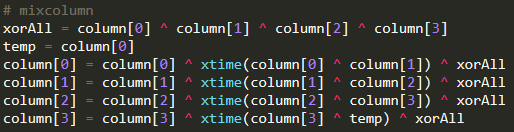
\includegraphics[width=1\linewidth]{images/mixcolumn.png}
  \caption{Core}
  \label{fig:core}
\end{subfigure}
\begin{subfigure}{.35\textwidth}
  \centering
  %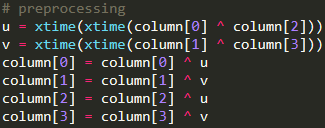
\includegraphics[width=1\linewidth]{images/preprocessing.png}
  \caption{Preprocessing}
  \label{fig:preprocessing}
\end{subfigure}
\caption{Mix columns base functions}
\label{fig:MixColumns}
\end{figure}
 
%----------------------------------------------------------------------------------------
%	SECTION 4
%----------------------------------------------------------------------------------------

\section{Use of Elliptic Curves in Cryptography}


%----------------------------------------------------------------------------------------
%	SECTION 5
%----------------------------------------------------------------------------------------

\section{Conclusion}

Even if the implementation proposed is much slower than the standard library chosen as comparison, it works well and it does its dirty job. The code may not be much optimized or it can have been written in a better way but my knowledge in python is not so huge, but this was an opportunity to dust and improve my experience.


%----------------------------------------------------------------------------------------
%	BIBLIOGRAPHY
%----------------------------------------------------------------------------------------

\bibliographystyle{abbrv}

%\bibliography{sample}

%----------------------------------------------------------------------------------------


\end{document}